 \subsubsection{UC11 - Visualizzazione delle informazioni utente}
 \begin{figure}[h]
 	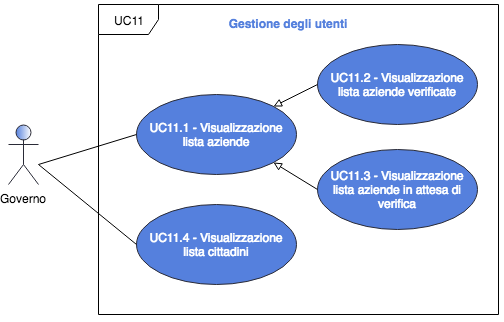
\includegraphics[width=9cm]{res/images/UC11.png}
 	\centering
 	\caption{UC11 - Visualizzazione delle informazioni utente}
 	
 \end{figure}
 \begin{itemize}
 	\item \textbf{Attori Primari}: governo;
 	\item \textbf{Descrizione}: il governo può accedere alle informazioni riguardanti:
 	\begin{itemize}
 		\item le aziende ed i cittadini registrati alla piattaforma;
 		\item le aziende che hanno effettuato la richiesta di registrazione;
 	\end{itemize}
 	\item \textbf{Scenario principale}: il governo accede alle informazioni riguardanti gli utenti della piattaforma ed alle eventuali relative operazioni disponibili;

 	\item \textbf{Precondizione}: il sistema riconosce che l'utente è autenticato con privilegi governativi e mostra le pagine utili alla ricerca di informazioni sugli utenti;
 	
 	\item \textbf{Postcondizione}: il governo ottiene dal sistema le liste degli utenti con le eventuali operazioni disponibili.
 \end{itemize}
 \subsubsection{UC11.1 - Visualizzazione lista aziende}
 \begin{itemize}
 	\item \textbf{Attori Primari}: governo;
 	\item \textbf{Descrizione}: il governo accede alla lista delle aziende, nella quale vengono mostrate tutte le informazioni utili ed operazioni disponibili. In particolare avviene la visualizzazione:
 	\begin{itemize}
 		\item della chiave\glosp Ethereum;
 		\item del nome;
 		\item della partita IVA;
 		\item sede dell'azienda (indirizzo);
 	\end{itemize}
 	\item \textbf{Scenario principale}: il governo vuole visualizzare la lista di tutte le aziende:
 	\begin{enumerate}[label=\alph*.]
 		\item iscritte alla piattaforma, con le relative informazioni riguardanti l'IVA [UC11.2];
 		\item che attualmente hanno fatto richiesta di registrazione alla piattaforma, ed eventualmente gestirne la richiesta [UC11.3];
 	\end{enumerate}
	\item \textbf{Specializzazione}:
	\begin{itemize}
	 	\item \textbf{UC11.2}: il governo vuole ottenere le informazioni relative alle aziende che sono già registrate alla piattaforma. In questo caso saranno presenti anche delle informazioni riguardati la situazione IVA delle aziende;
	 	\item \textbf{UC11.3}: il governo vuole ottenere le informazioni relative alle aziende che sono in attesa di essere approvate. Da questa vista verranno offerte al governo le operazioni di approvazione/rigetto della richiesta;
	\end{itemize}
 	\item \textbf{Precondizione}: il governo ha richiesto le informazioni relative alle aziende;
 	\item \textbf{Postcondizione}: il governo ottiene dal sistema la lista delle aziende cercate, con le relative operazioni disponibili.
\end{itemize}
\subsubsection{UC11.2 - Visualizzazione lista aziende registrate}
 \begin{itemize}
	\item \textbf{Attori Primari}: governo;
	\item \textbf{Descrizione}: il governo visualizza la lista delle aziende registrate alla piattaforma. Per ogni azienda è reso disponibile, oltre alle informazioni di base [UC11.1], lo stato del pagamento del saldo IVA, ovvero può controllare se l'azienda risulta:
	\begin{itemize}
		\item \textbf{insolvente}: non ha ancora provveduto alla liquidazione IVA di almeno uno dei trimestri precedenti entro i termini fissati;
		\item \text{in fase di pagamento}: l'azienda deve ancora effettuare il versamento IVA riguardante l'ultimo trimestre, ed i termine del pagamento non è ancora scaduto. Nei trimestri antecedenti la situazione risulta "regolare";
	    \item \textbf{in dilazione}: in caso l'azienda abbia richiesto il pagamento dilazionato del saldo IVA a debito ed il termine della dilazione non è ancora scaduto;
		\item \textbf{regolare}: l'azienda ha provveduto al pagamento del saldo IVA a debito del trimestre precedente oppure ha ricevuto il rimborso nel caso in cui sia risultata "In attesa di rimborso" nel trimestre precedente;
		\item \textbf{in attesa di rimborso}: nel trimestre precedente il saldo IVA è risultato a credito, e non è ancora stato effettuato il rimborso;
	\end{itemize}
	L'azienda può ricadere in uno solo trai casi sopra descritti. Lo stato di insolvenza di un trimestre precedente, ha la predominanza sugli stati dei trimestri successivi ad esso.
	\item \textbf{Scenario principale}: il governo richiede la lista delle aziende registrate e  già verificate;
	\item \textbf{Precondizione}: il sistema riconosce che l'utente è autenticato con privilegi governativi ed ha richiesto di ottenere la lista di tutte aziende già verificate;
	\item \textbf{Postcondizione}: il governo ottiene dal sistema la lista delle aziende registrate e verificate, con associate le operazioni che può effettuare su di esse.
\end{itemize}
\subsubsection{UC11.3 - Visualizzazione lista aziende in attesa di verifica}

\begin{itemize}
	\item \textbf{Attori Primari}: governo;
	\item \textbf{Descrizione}: il governo ottiene la lista delle aziende che sono in attesa di essere verificate per poter poi usufruire della piattaforma. Per ognuna di esse avrà la possibilità di accettare o rifiutare la richiesta;
	\item \textbf{Scenario principale}: il governo richiede la lista delle aziende che sono in attesa di essere verificate;
	\item \textbf{Precondizione}: il sistema riconosce che l'utente è autenticato con privilegi governativi ed ha richiesto di ottenere la lista di tutte le aziende in attesa di verifica;
	\item \textbf{Postcondizione}: il governo ottiene dal sistema la lista delle aziende in attesa di verifica, con associate le operazioni che può effettuare su di esse.
\end{itemize}
\subsubsection{UC11.4 - Visualizzazione lista cittadini}
\begin{itemize}
	\item \textbf{Attori Primari}: governo;
	\item \textbf{Descrizione}: il governo ottiene la lista dei cittadini. Per ognuno di essi può eseguire:
	\begin{itemize}
		\item visualizzazione della chiave\glosp Ethereum;
		\item visualizzazione del nome;
		\item visualizzazione del cognome;
		\item visualizzazione della codice fiscale;
		\item visualizzazione dell'indirizzo di residenza;
	\end{itemize}
	\item \textbf{Scenario principale}: il governo richiede la lista dei cittadini. Per ognuno di essi visualizza alcune informazioni;
	\item \textbf{Precondizione}: il sistema riconosce che l'utente è autenticato con privilegi governativi ed ha richiesto di ottenere la lista di tutti i cittadini;
	\item \textbf{Postcondizione}: il governo ottiene dal sistema la lista dei cittadini, con associate le operazioni che può effettuare su di essi.
\end{itemize}
